\documentclass[10pt,twocolumn,letterpaper]{article}

\usepackage{cvpr}
\usepackage{times}
\usepackage{epsfig}
\usepackage{graphicx}
\usepackage{amsmath}
\usepackage{amssymb}

\makeatletter
\renewcommand{\paragraph}{%
  \@startsection{paragraph}{4}%
  {\z@}{0.5ex \@plus 1ex \@minus .2ex}{-1em}%
  {\normalfont\normalsize\bfseries}%
}
\makeatother
% Include other packages here, before hyperref.

% If you comment hyperref and then uncomment it, you should delete
% egpaper.aux before re-running latex.  (Or just hit 'q' on the first latex
% run, let it finish, and you should be clear).
\usepackage[breaklinks=true,bookmarks=false]{hyperref}

\cvprfinalcopy % *** Uncomment this line for the final submission

\def\cvprPaperID{****} % *** Enter the CVPR Paper ID here
\def\httilde{\mbox{\tt\raisebox{-.5ex}{\symbol{126}}}}

% Pages are numbered in submission mode, and unnumbered in camera-ready
%\ifcvprfinal\pagestyle{empty}\fi
\setcounter{page}{1}
\begin{document}

%%%%%%%%% TITLE
\title{Deep Reinforcement Learning for Autonomous Systems}

\author{Piero Macaluso - s252894\\
    Candidate\\
    Politecnico di Torino\\
    % For a paper whose authors are all at the same institution,
    % omit the following lines up until the closing ``}''.
    % Additional authors and addresses can be added with ``\and'',
    % just like the second author.
    % To save space, use either the email address or home page, not both
    \and
    Prof. Pietro Michiardi\\
    Supervisor\\
    EURECOM\\
    \and
    Prof. Elena Baralis\\
    Supervisor\\
    Politecnico di Torino\\
}

\maketitle
%\thispagestyle{empty}

%%%%%%%%% ABSTRACT
% \begin{abstract}
%   The ABSTRACT is to be in fully-justified italicized text, at the top
%   of the left-hand column, below the author and affiliation
%   information. Use the word ``Abstract'' as the title, in 12-point
%   Times, boldface type, centered relative to the column, initially
%   capitalized. The abstract is to be in 10-point, single-spaced type.
%   Leave two blank lines after the Abstract, then begin the main text.
%   Look at previous CVPR abstracts to get a feel for style and length.
%\end{abstract}

\textit{This document represents the summary of the master thesis project. The source code of this work is publicly available at \url{https://github.com/pieromacaluso/Deep-RL-Autonomous-Systems}}
%%%%%%%%% BODY TEXT
\section{Introduction}

Because of its potential to thoroughly change mobility and transport, autonomous systems and self-driving vehicles are attracting much attention from both the research community and industry.
Recent work has demonstrated that it is possible to rely on a comprehensive understanding of the immediate environment while following simple high-level directions, to obtain a more scalable approach that can make autonomous driving a ubiquitous technology.
However, to date, the majority of the methods concentrates on deterministic control optimisation algorithms to select the right action, while the usage of deep learning and machine learning is entirely dedicated to object detection and recognition.

Recently, we have witnessed a remarkable increase in interest in Reinforcement Learning (RL). It is a machine learning field focused on solving Markov Decision Processes (MDP), where an agent learns to make decisions by mapping situations and actions according to the information it gathers from the surrounding environment and from the reward it receives, trying to maximise it.
As researchers discovered, it can be surprisingly useful to solve tasks in simulated environments like games and computer games, and it showed encouraging performance in tasks with robotic manipulators. Furthermore, the great fervour produced by the widespread exploitation of deep learning opened the doors to function approximation with convolutional neural networks, developing what is nowadays known as deep reinforcement learning.

\subsection{Objective}

In this thesis, we argue that the generality of reinforcement learning makes it a useful framework where to apply autonomous driving to inject artificial intelligence not only in the detection component but also in the decision-making one.
The focus of the majority of reinforcement learning projects is on a simulated environment. However, a more challenging approach of reinforcement learning consists of the application of this type of algorithms in the real world.

After an initial phase where we studied the state-of-the-art literature about reinforcement learning and analysed the set of possible alternatives about technologies to use, we started our project starting from the ideas contained in \cite{kendall2019learning}, where the authors were able to train a self-driving vehicle by using Deep Deterministic Policy Gradient (DDPG) \cite{lillicrap2015continuous} by tuning hyper-parameters in simulation.
Our approach was different: we researched an algorithm which suitable for real-world experiments and able to operate correctly without an expensive real-world hyper-parameter tuning made in simulators.
We found in Soft Actor-Critic (SAC) \cite{haarnoja2018soft} the algorithm we needed.

Therefore, our thesis consisted of two main contributions:
\begin{enumerate}
    \item Designing of the Control System to let all components and technologies involved interact.
    \item Setting up the experimental framework with SAC algorithm and carrying out an experiment to analyse the strengths and weaknesses of this approach.
\end{enumerate}


% For this reason, we designed and implemented a control system for Cozmo, a small toy robot developed by Anki company, by exploiting the Cozmo SDK and OpenAI Gym to build up a standardised environment in which to apply any reinforcement learning algorithm. This implementation represents the first contribution of our thesis. The second contribution of our work consists of the implementation of Soft Actor-Critic (SAC), a model-free reinforcement learning algorithm suitable for real-world experiments, to solve the self-driving task. During the test phase, the robot reached a maximum of more than 3 meters before the human intervention, succeeding in completing the track. However, the mean value we obtained is about 1 metre over 10 test episodes. Because of the instability of the results obtained, we focused on strength and weaknesses of this approach outlining what could be next steps to make this cutting-edge technology concrete and efficient.

%-------------------------------------------------------------------------
\section{Design of the control system}

We based our project on Cozmo, a little toy robot produced by Anki, whose developers offered a granular and fully-featured Python SDK with many interfaces to allow direct control of the robot.
We found it to be suitable for our experimental needs: it mounts a grayscale camera with 60 FOV and has two tracks to steer and drive.
We aimed to apply deep reinforcement learning algorithms, so we decided to use PyTorch as deep learning framework and the standardised approach provided by OpenAI Gym to build up the reinforcement learning environment for the experiment.

Our idea was to build a system where the human holds complete control over the experiment progress: he can start the episode and suspend it when the robot reaches a fatal state to reposition it in the closest stable situation and restart the loop.
In this scenario, the human has total responsibility for the robot training: he is the one who decides when an action is dangerous or not by disengaging reinforcement learning algorithms decision.

\begin{figure}[tbp]
    \centering
    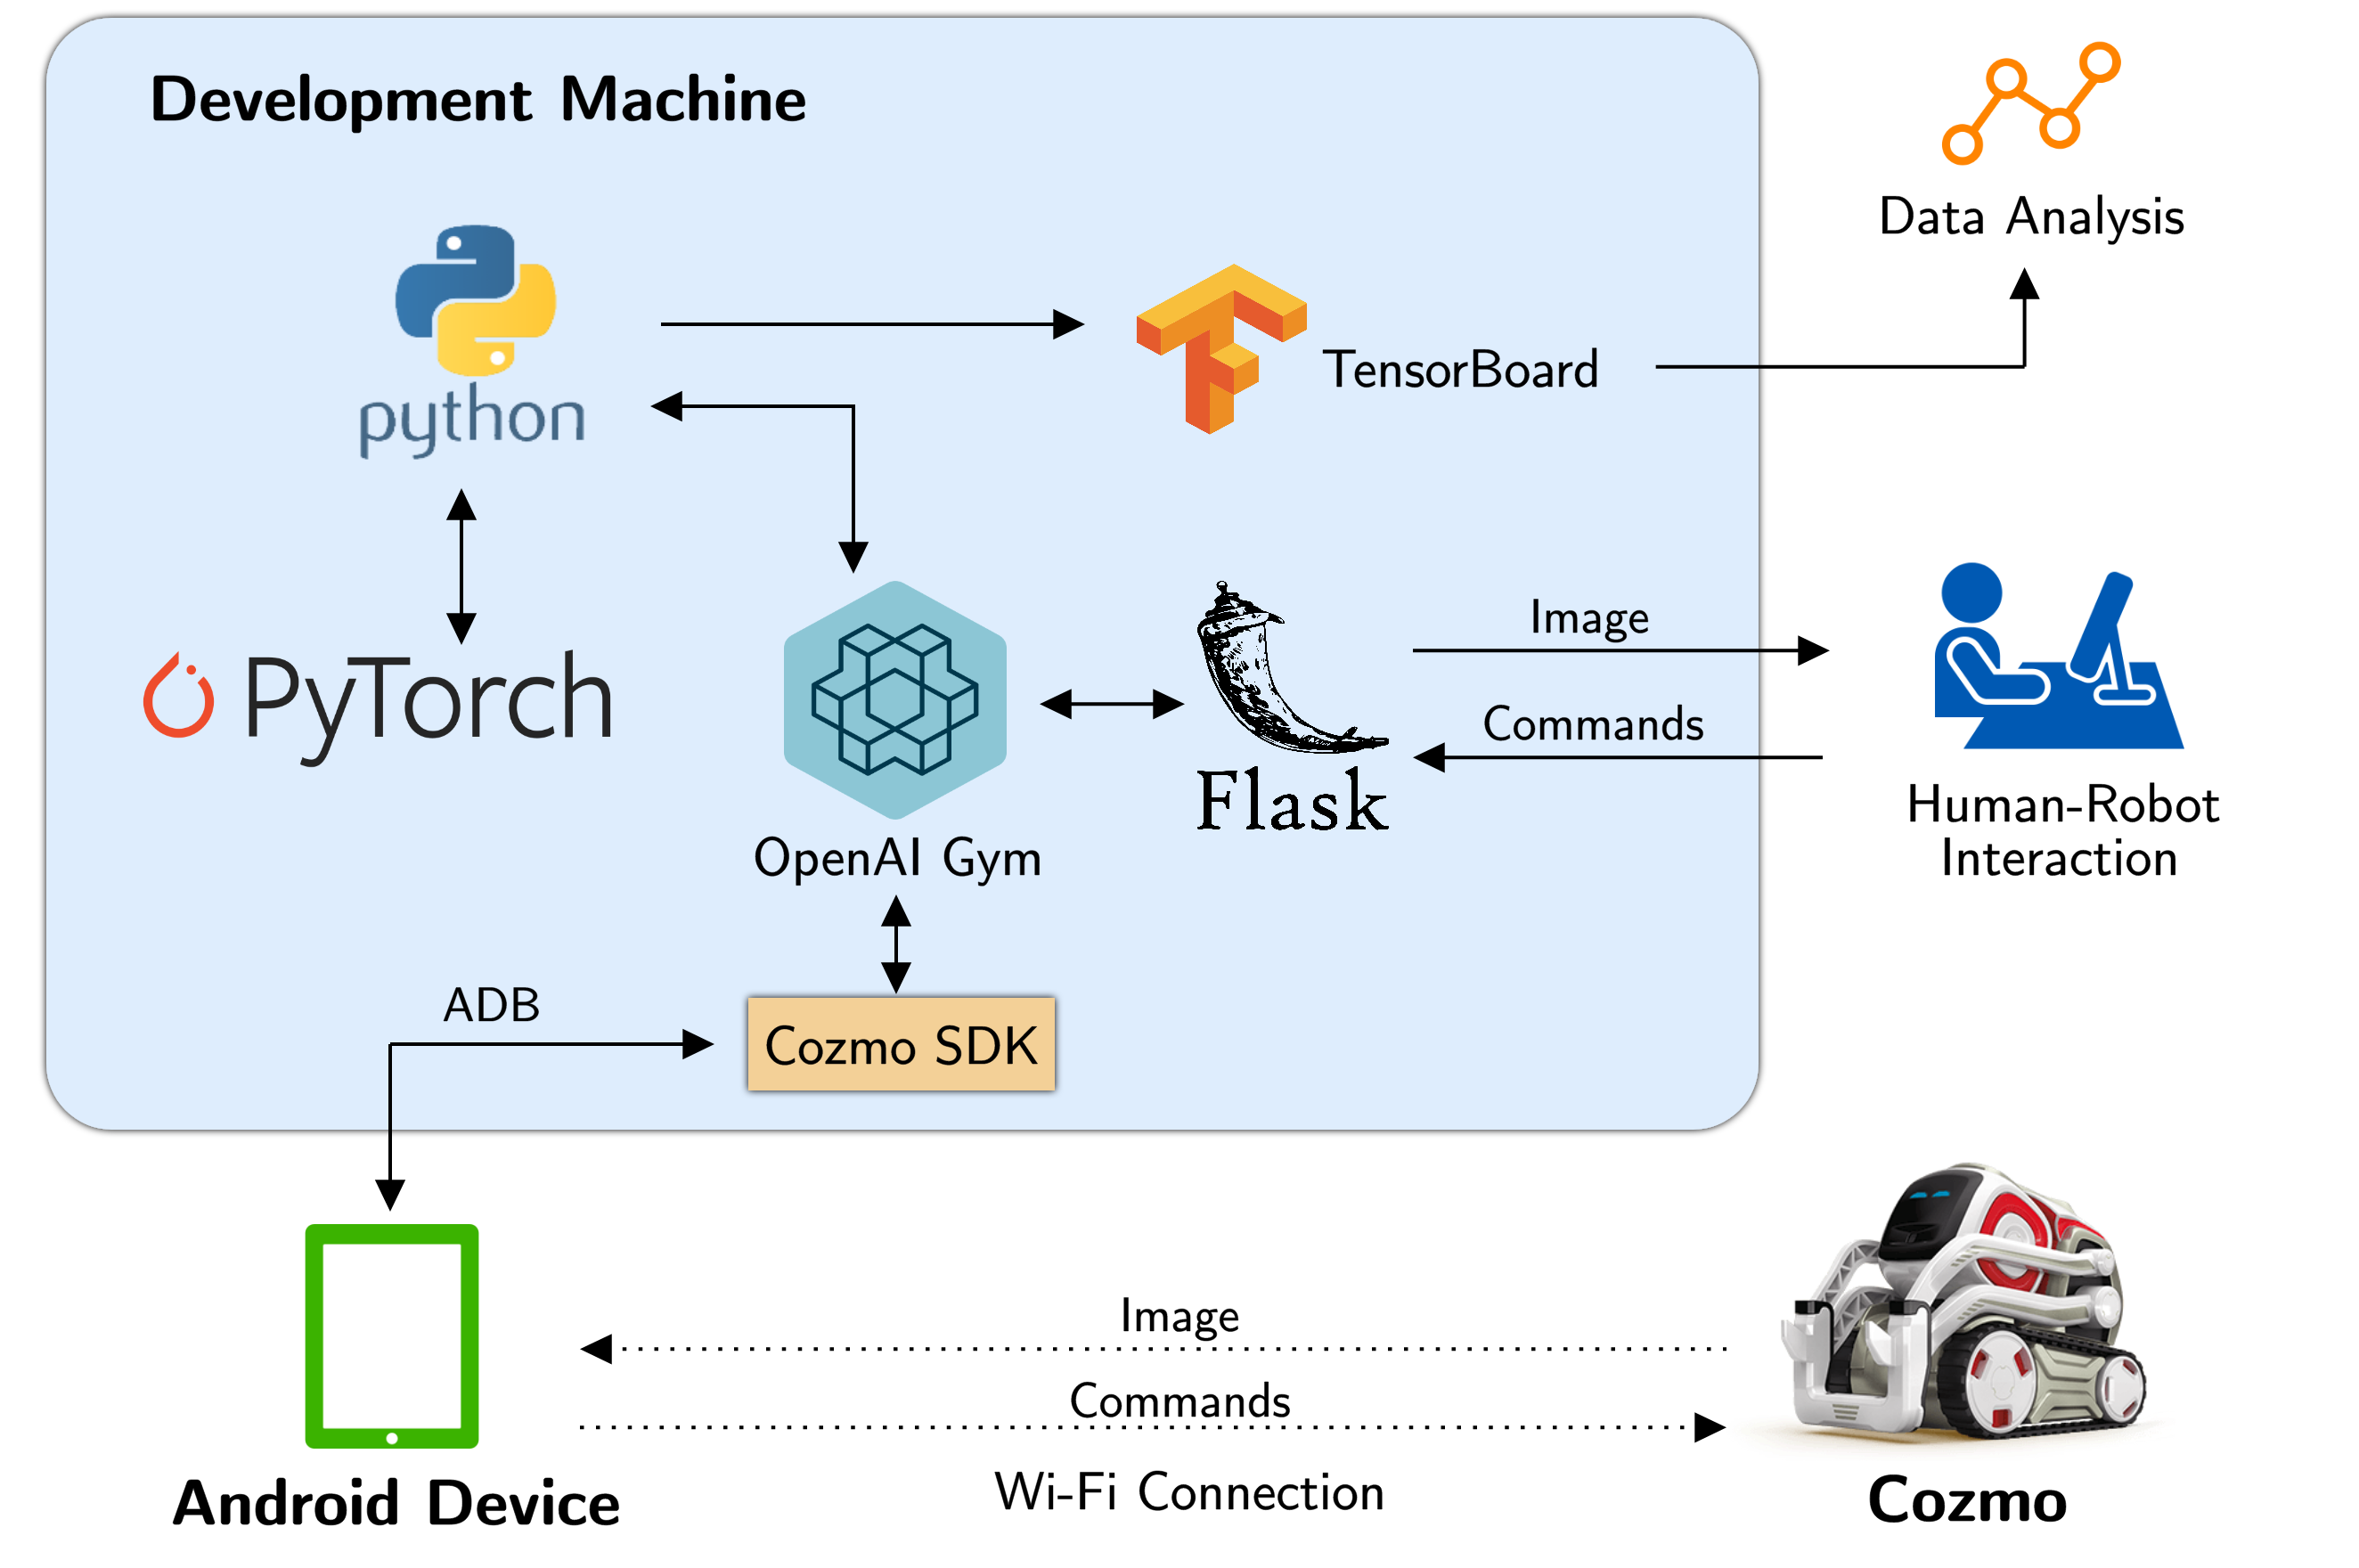
\includegraphics[width=0.97\columnwidth]{cozmo-system.png}
    \caption[Outline of the control system]{Outline of the control system that shows the most crucial technologies and component involved.}
    \label{system}
\end{figure}

To obtain this configuration, we managed to design a simple and intuitive user interface that prompts the user when a new experiment starts. This interface provides a live stream from Cozmo on-board camera and a set of keys with the related function. It works through Javascript to communicate to a Flask server that interfaces directly to Cozmo SDK and the OpenAI Gym environment to provide information for the user (e.g.\ images, learning information) and the robot (e.g.\ commands). We used TensorBoard to gather data for posterior analysis and representations. The outline of the system we obtained is available in figure \ref{system}.

% TODO: Grammarly error
\textit{CozmoDriver-v0} is the Cozmo environment we designed. It represents the result of continuous development and testing to solve all the problems and particularities that we have found along the way. We implemented all the requirements and needs dictated by the type of experiment, putting in place all the compromises to manage the available RAM and make experiments manageable by reducing the learning time between one episode and the next one.
One of the most crucial features we implemented is the rescue system, useful in a context where experiments last tens of hours and unexpected errors can occur.
It consists of two main part. The first one is a volatile backup system: it stores the state status before the episode to allow the user to restore it in case of a broken episode. The second one is a checkpoint system to save the state of the experiment and allow the user to restore it in the following days.
%

We spent some time to search for the most reliable way to build a transportable track where to train Cozmo efficiently without influencing it through the presence of reflections, but providing a path as close as possible to reality.
We also designed it by using grey cotton fabric as a baseline and a white paper tape of width equal to $2.5$cm to draw the lane.

Before starting the experiment, we formalised the problem as an MDP obtaining the following setup:

\paragraph{State Space} The current state observation consists of two $64 \times 64$ grayscale images which represent the situation before and after the action respectively. We decided to resize images provided by Cozmo SDK for memory reason due to the experience replay memory needed for off-policy algorithms.

\paragraph{Action Space} We used a vector of two real value to represent how the robot can interact with the surrounding environment: the first value represents the desired speed with a range between 0 and 1, while the second one describes the vehicle steer with a range between -1 and 1. Both values are the result of a simplification useful in the learning phase. In practice, the system designed converts these values to correctly interact with the robot. The maximum speed reachable is 150mm/s.

\paragraph{Reward Function}. The reward function defines which is the purpose of the task to solve. After an analysis of the literature available, we decided to formalise this function as the total length of track crossed by the robot after each action taken. Despite its simple formulation, this choice revealed to be effective.
Furthermore, this choice leads to match reward with length covered, useful fact to support the developer in quantifying agent improvements and have better feedback.

\section{Experiments}

The path that led to the final implementation of the algorithm allowed us to detect some specific requirements and to overcome them with appropriate countermeasures.
We decided to firstly implement a simplified environment to test functionalities and reinforcement learning algorithms we aimed to use in Cozmo environment. We used the inverted pendulum swing-up problem, a classic problem in the control literature and available in OpenAI Gym. 
The original implementation of this environment consisted of observations with values related to the current angle and speed of the pendulum. For this reason we decided to build a wrapper for the original environment in order to receive observations as raw pixels, since the goal was to apply the same considerations and the same convolutional neural networks that we would use in the Cozmo environment.

The results of the experiments carried out using hyper-parameters taken from the available literature, showed that SAC algorithm has a better performance than the DDPG one, both in terms of stability and number of episodes to achieve a working policy. Therefore, we decided to implement SAC algorithm to carry out experiments in the Cozmo environment.

We opted for a neural network with three convolutional layers with 16 features of 3$\times$3 dimension, a stride of 2, zero padding with two fully-connected layers with a hidden size of 256 features in the last part
We applied batch normalisation after each convolutional level and Rectified Linear Unit function (ReLU) as non-linearity.

We managed to complete a whole set of 3000 episodes exploiting the SAC algorithm to solve the autonomous driving task with Cozmo.
Taking into account waiting times between episodes and charging times, we managed to complete the experiment in almost one working week, after almost $1.3\times 10^5$ epochs of learning.

\begin{figure}[tbp]
    \centering
    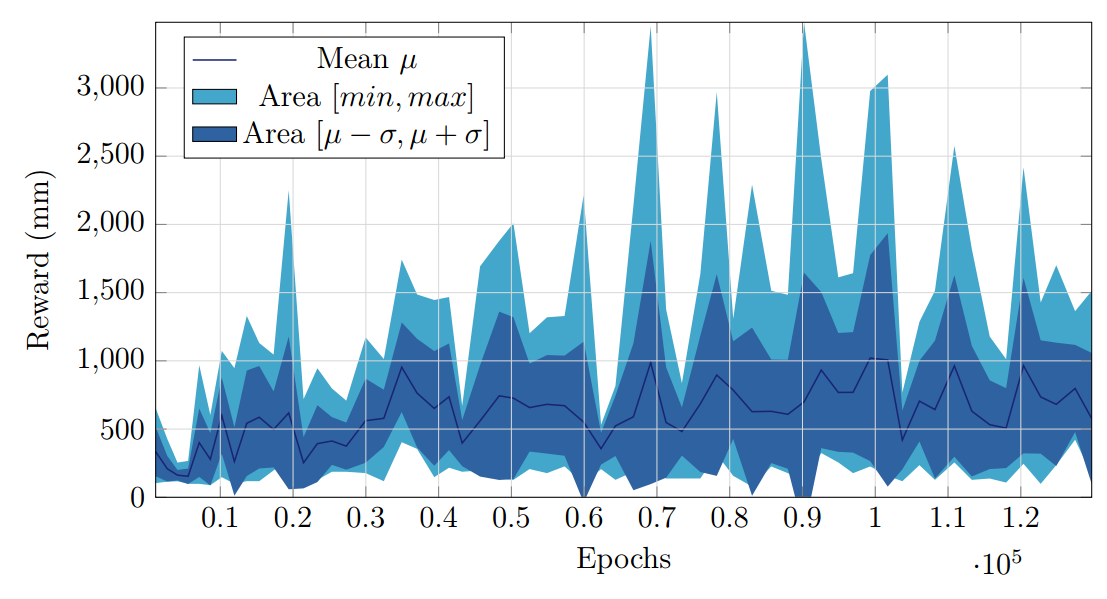
\includegraphics[width=0.97\columnwidth]{test_confidence.png}
    \caption[SAC CozmoDriver-v0 Test Average Reward Plot]{SAC CozmoDriver-v0 Test Average Reward Plot. The graph reports mean, standard deviation range and min-max range of the average reward obtained from 10 test episodes every 50 episodes.}
    \label{confidence}
\end{figure}

The agent reached the most crucial results in the testing phase presented in figure \ref{confidence} where we plotted minimum and maximum values obtained in every set of ten episode together with the mean and the standard deviation.
Following this approach we noticed a performance increase with a maximum mean reached of almost 1 metre.
Furthermore, the maximum value reached among all tests episodes was equal to almost 3.5 metres which equals more than one complete tour of the track.
It is noticeable that the results are not stable as we expected from the experiments with the inverted pendulum environment: the reward values do not improve uniformly with increasing epochs.
However, carrying out the experiments episode by episode, we noticed a marked improvement in the performance obtained in the tests. The robot learned to approach turns and to stay on the lane of a straight road.

\section{Conclusions}

The plot reports a visible improvement in the maximum length of track traveled before the disengagement of the user.
Despite these improvements, the agent was not able to learn how to drive in a secure and stable way, as we can notice from the unstable growth of the mean reward.
These facts made us reflect on the critic points of our experiment setup that may have had a role in the instability of the results obtained.

We localised two major problems which, in our opinion, have had a particular influence on the results obtained.
The first factor was the amount of RAM available in the development machine. This limitation forced us to decrease the size of the replay memory and a consequent early deletion of less recent episodes. Analysing the plots, we noticed that this fact translated in the increase of the temperature parameter: this symptom underlines the need for the algorithm to explore more the solution space.
The second major problem was the limitation of the camera sensor on the robot, particularly its viewing angle. The features offered by the Anki Cozmo camera proved to be inadequate to observe the track we designed.
We noticed this fact after many episodes when the robot started to improve its performance: it began to adopt a wave behaviour on the straights, interpreting the vision of a single road line as a curve.

\subsection{Future Work}

Our proposals about future improvements to the project grow from the weakness in our approach.
It could be interesting to execute these algorithms on a device with a bigger RAM, but also to design this approach with a Variational Auto-Encoder (VAE) to reduce the dimensionality of the information retrieved during experiments.

It may be useful to enhance sensors installed in the self-driving robot.
A possible alternative to Anki Cozmo could be Anki Vector, the successor of Cozmo which mounts a 720p camera with 120 Ultra Wide FOV or to build up a personal \textit{Donkey Car} with custom specifications.
Anki Vector could be interesting to perform reinforcement learning algorithms with the usage of the renewed front camera together with the infrared laser scanner on-board to investigate approaches to data fusion with more sensors.

Another intriguing research path consists of an investigation about the application of model-based reinforcement learning algorithms to autonomous driving.
A more in-depth review of the literature to better understand the feasibility of this approach, focusing on its strengths and weaknesses compared to model-free ones can be the right starting point.

{\footnotesize
    \bibliographystyle{abbrv}
    \bibliography{egbib}
}

\end{document}
